%!TeX program = xelatex
%
% $Header: https://metis.ipfn.ist.utl.pt/svn/cdaq/Users/Bernardo/Aulas/EUROPhD/teXfiles/MagDiag/MagDiagApplause.tex 12911 2018-09-26 17:44:08Z bernardo $
%
%% SVN keywords
%% $Author: bernardo $
%% $Date: 2018-09-26 18:44:08 +0100 (Wed, 26 Sep 2018) $
%% $Revision: 12911 $
%% $URL: https://metis.ipfn.ist.utl.pt/svn/cdaq/Users/Bernardo/Aulas/EUROPhD/teXfiles/MagDiag/MagDiagApplause.tex $
%%
\documentclass{beamer}
%\documentclass[handout]{beamer}
\usepackage{pgfpages}
%\pgfpagesuselayout{2 on 1}[a4paper,border shrink=5mm] % for instance
%If there is something you do not want on the handout, add | handout:0 to the overlay specification. So
%\only<1-3| handout:0>{foo}
%
% Compile this file with XeLateX
% Compiled  in 2018/09/26
%   XeTeX, Version 3.14159265-2.6-0.99999 (MiKTeX 2.9.6800 64-bit)
%
% If you have compilation problems Delete the .nav and .toc files
% https://tex.stackexchange.com/questions/352017/miktex-and-beamer-error-beamerendinputifotherversion
%
% This file is a solution template for:
% - Talk at a conference/colloquium.
% - Talk length is about 20min.
% - Style is ornate.

\usepackage{hyperref}

\usepackage[siunitx]{circuitikz}
\usepackage{tikz}
\usetikzlibrary{shapes.arrows}


\tikzset{
    myarrow/.style={
        draw,
        fill=orange,
        single arrow,
        minimum height=3.5ex,
        single arrow head extend=1ex
    }
}
\newcommand{\arrowup}{%
\tikz [baseline=-0.5ex]{\node [myarrow,rotate=90] {};}
}
\newcommand{\arrowdown}{%
\tikz [baseline=-1ex]{\node [myarrow,rotate=-90] {};}
}

\newcommand{\arrowright}{%
\tikz [baseline=-1ex]{\node [myarrow,rotate=0] {};}
}


\mode<presentation>
{
  \usetheme{Warsaw} %Warsaw Frankfurt Madrid
  % or ...
  \setbeamercovered{transparent}
  % or whatever (possibly just delete it)
}


\usecolortheme{crane} % beetlealbatross

%http://tex.stackexchange.com/questions/73718/frame-numbering-in-warsaw-theme
\setbeamercolor{mycolor}{fg=red,bg=olive}
\defbeamertemplate*{footline}{shadow theme}{%
\leavevmode%
\hbox{\begin{beamercolorbox}[wd=.5\paperwidth,ht=2.5ex,dp=1.125ex,leftskip=.3cm plus1fil,rightskip=.3cm]{author in head/foot}%
    \usebeamerfont{author in head/foot}\hfill\insertshortauthor
\end{beamercolorbox}%
\begin{beamercolorbox}[wd=.4\paperwidth,ht=2.5ex,dp=1.125ex,leftskip=.3cm,rightskip=.3cm plus1fil]{title in head/foot}%
    \usebeamerfont{title in head/foot}\insertshorttitle\hfill%
\end{beamercolorbox}%
\begin{beamercolorbox}[wd=.1\paperwidth,ht=2.5ex,dp=1.125ex,leftskip=.3cm,rightskip=.3cm plus1fil]{mycolor}%
\hfill\insertframenumber\,/\,\inserttotalframenumber
\end{beamercolorbox}}%
\vskip0pt%
}

\usepackage[english]{babel}
% or whatever

%\usepackage[latin1]{inputenc}
\usepackage[utf8]{inputenc} % set input encoding (not needed with XeLaTeX)
% or whatever

\usepackage{times}
\usepackage[T1]{fontenc}
% Or whatever. Note that the encoding and the font should match. If T1
% does not look nice, try deleting the line with the fontenc.

%emoticons in LaTeX
\usepackage{wasysym}
%\smiley
%\frownie

%\title[Magnetic Diagnostics for Plasmas, APPLAuSE, European PhD]{Magnetic Diagnostics for Plasmas}
\title[Magnetic Diagnostics, IAEA fusion training course]{Magnetic Diagnostics for Plasmas}

%\subtitle{CURRICULAR UNIT: Methodologies \& Techniques}

\author[B.~Carvalho, 25 July 2019] % (optional, use only with lots of authors)
{\href{mailto:bernardo.carvalho@tecnico.ulisboa.pt}{\nolinkurl{bernardo.carvalho@tecnico.ulisboa.pt}} }
% \inst{1}  \and S.~Another\inst{2}
% - Give the names in the same order as the appear in the paper.
% - Use the \inst{?} command only if the authors have different
%   affiliation.

%\institute[I. S Técnico] % (optional, but mostly needed)
%{
%  \inst{1}%
%  Department of Physics\\
%  Instituto Superior Técnico -
%  University of Lisbon
%  \and
%  \inst{2}%
%  Instituto de Plasmas e Fusão Nuclear\\
%}
% - Use the \inst command only if there are several affiliations.
% - Keep it simple, no one is interested in your street address.

\date[APPLAuSE 2018] % (optional, should be abbreviation of conference name)
{\small APPLAuSE Advanced Program in Plasma Science and Engineering
% Joint Research Doctorate in Fusion Science and Engineering \\
% 
\includegraphics[width=0.25 \columnwidth]{figures/unipd_logo2.png}
}
% - Either use conference name or its abbreviation.
% - Not really informative to the audience, more for people (including
%   yourself) who are reading the slides online

\subject{Plasma Science and Engineering}
% This is only inserted into the PDF information catalog. Can be left
% out.

% If you have a file called "university-logo-filename.xxx", where xxx
% is a graphic format that can be processed by latex or pdflatex,
% resp., then you can add a logo as follows:

 \pgfdeclareimage[height=0.5cm]{logo-ist}{logo-ist}
 \logo{\pgfuseimage{logo-ist}}

% Delete this, if you do not want the table of contents to pop up at
% the beginning of each subsection:
%\AtBeginSubsection[]
%{
%  \begin{frame}<beamer>{Outline}
%    \tableofcontents[currentsection,currentsubsection]
%  \end{frame}
%}


\AtBeginSection[] % Do nothing for \section*
{
\begin{frame}<beamer>
\frametitle{Outline}
	\tableofcontents[currentsection]
\end{frame}
}

% If you wish to uncover everything in a step-wise fashion, uncomment
% the following command:

%\beamerdefaultoverlayspecification{<+->}


\begin{document}
\setbeamertemplate{caption}{\insertcaption}
%\setbeamertemplate{caption}{%
%\begin{beamercolorbox}[wd=.5\paperwidth, sep=.2ex]{block body}\insertcaption%
%\end{beamercolorbox}%
%}

%\begin{frame}
%	\titlepage
%  \titlepage
%\end{frame}

\begin{frame}
\titlepage
\end{frame}

\begin{frame}{Outline}
  \tableofcontents
  % You might wish to add the option [pausesections]
\end{frame}


% Structuring a talk is a difficult task and the following structure
% may not be suitable. Here are some rules that apply for this
% solution:

% - Exactly two or three sections (other than the summary).
% - At *most* three subsections per section.
% - Talk about 30s to 2min per frame. So there should be between about
%   15 and 30 frames, all told.

% - A conference audience is likely to know very little of what you
%   are going to talk about. So *simplify*!
% - In a 20min talk, getting the main ideas across is hard
%   enough. Leave out details, even if it means being less precise than
%   you think necessary.
% - If you omit details that are vital to the proof/implementation,
%   just say so once. Everybody will be happy with that.
\section{Magnetic Diagnostics}
\subsection*{A Bit of History}
%\subsection{Portuguese Discoveries}
\begin{frame}{Portuguese Discoveries, XV - XVI Centuries}
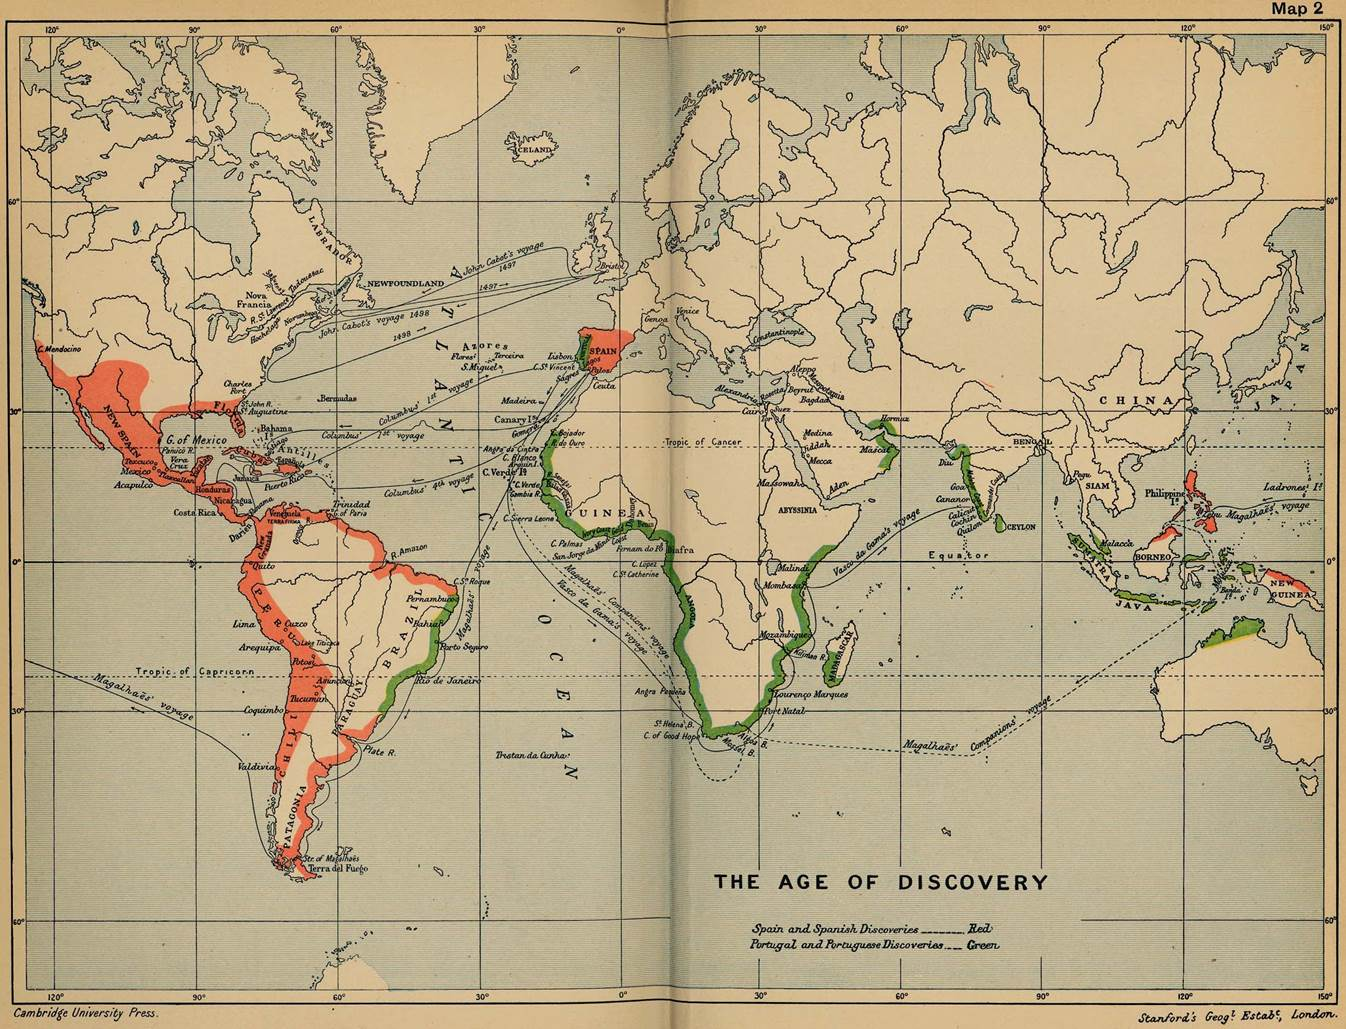
\includegraphics[width=8.5 cm]{discov}
\end{frame}

\begin{frame}{The Portuguese Heroes}

\begin{columns}
\column{0.2\textwidth}
	\begin{figure}[ht]
	\begin{center}
	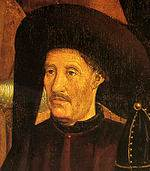
\includegraphics[width=0.9 \columnwidth]{Henry.jpg}
	%\setbeamerfont{caption name}{size=\tiny}
	\caption{\tiny Henry the Navigator 1394-1460}	 %\Large
	\end{center}
	\end{figure}
\column{0.2\textwidth}
	\begin{figure}[ht]
	\begin{center}
	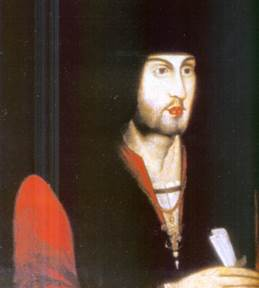
\includegraphics[width=0.9 \columnwidth]{JohnII.jpg}
    	\caption{\tiny King John II ~~~~~~~ 1455-1495}
%	\caption{King John II  1455-1495}
	\end{center}
	\end{figure}
\column{0.2\textwidth}
	\begin{figure}[ht]
	\begin{center}
	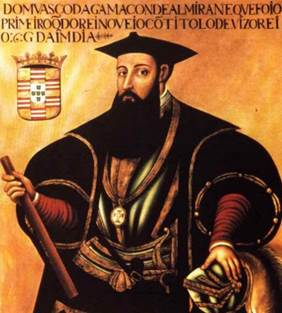
\includegraphics[width=0.9 \columnwidth]{Vasco.jpg}
	\caption{\tiny Vasco da Gama ~~~ 1460-1524}
%	\caption{\small Vasco da Gama ~~  1460-1524}
	\end{center}
	\end{figure}
\column{0.2\textwidth}
	\begin{figure}[ht]
	\begin{center}
	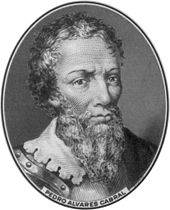
\includegraphics[width=0.9 \columnwidth]{Cabral.jpg}
	\caption{\tiny Pedro Alvares Cabral ~~ 1467-1520}
	\end{center}
	\end{figure}

\column{0.2\textwidth}
	\begin{figure}[ht]
	\begin{center}
	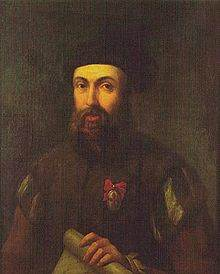
\includegraphics[width=0.9 \columnwidth]{Magellan.jpg}
	\caption{\tiny Ferdinand Magellan ~~ 1480 – 1521}
%	\parbox{0.9 \columnwidth}{\center Ferdinand Magellan, 1480–1521}
	\end{center}
	\end{figure}
\end{columns}

\end{frame}

\begin{frame}{The Instruments}
\begin{columns}
\column{0.33\textwidth}
	\begin{figure}[ht]
	\begin{center}
	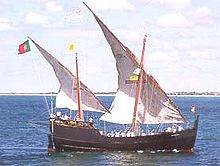
\includegraphics[width=0.9 \columnwidth]{Caravel.jpg}
	\caption{\tiny The Caravel}
	\end{center}
	\end{figure}
\column{0.33\textwidth}
	\begin{figure}[ht]
	\begin{center}
	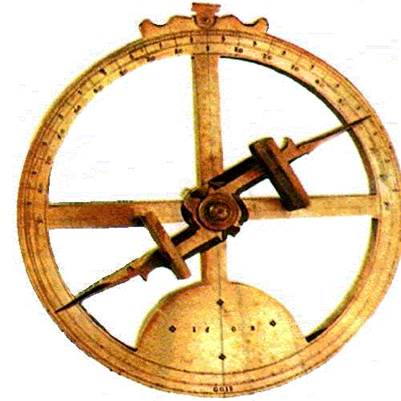
\includegraphics[width=0.9 \columnwidth]{Astrolab.jpg}
	\caption{\tiny The Astrolabe}
	\end{center}
	\end{figure}
\column{0.33\textwidth}
 \visible<2->  {
 	\begin{figure}[ht]
	\begin{center}
	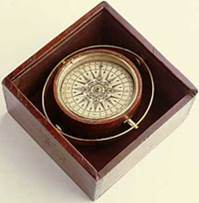
\includegraphics[width=0.9 \columnwidth]{Compass.jpg}
	\caption{\tiny The Compass}
	\end{center}
	\end{figure}
}
\end{columns}
\end{frame}

%%%%%%%%%%%%%%%%%%%%%%
\subsection{General Principles}

\begin{frame}{ Magnetic Diagnostics: General Principles}%{Subtitles are optional.}
    Magnetic measurements provide some of the most   \alert{fundamental} and %fundamental
\alert{essential} information about a fusion plasma:

  \begin{itemize}
  \item<2->
    $I_{plasma}$, Internal Inductance $\ell_i$,   Position and Speed of current centroid,
	Boundary Shape, Thermal Energy, Currents in the magnet coils,
	and the strength of the magnetic fields confining the plasma.
%
%    Use \texttt{itemize} a lot.
  \item<3->
    Information about the internal characteristics of the plasma and
	about asymmetries caused by large-scale MHD instabilities.
  \item<4-> Halo Currents in machine structures.
  \end{itemize}
\end{frame}

\begin{frame}{General Principles II}%{Subtitles are optional.}
  \begin{itemize}
  \item Essential for \alert{Equilibrium}  Reconstructions
   \begin{itemize}
		\item Post-discharge full equilibrium codes
		\item Real-Time Plasma Shape and Position Control
  \end{itemize}
  \item<2-> Magnetic diagnostics are external, passive and \alert{ ROBUST}!
   \begin{itemize}
		\item The measurements remain valid and useful over the full range of
		plasma density and temperature as well as during large transient events (disruptions).
  \end{itemize}
  \end{itemize}
\end{frame}

\begin{frame}{Axisymmetric Configuration of Fusion Devices}{Magnetic field}

\begin{columns}
\column{0.7\textwidth}
   \begin{itemize}
   \item In a cylindrical coordinate system,  $(R, Z, \phi)$,   $\vec{B}$
   can be expressed in terms of two scalar functions, $F$, and $\Psi$:
    \begin{equation*}%\label{eq:mag_axis}
		 \vec{B} =  (F \,  \hat{\phi}  + \nabla \Psi \times \hat{\phi} )/ R
		 % E(u) = \int |\nabla u|^2 dx
	\end{equation*}
	\item<2-> $\vec{B}$ field can be separated in
		\begin{itemize}
			\item Toroidal Field: $\vec{B}_{\phi} = \frac{F}{R}\, \hat{\phi} $
			\item Poloidal Field: $\vec{B}_{p} = \frac{\nabla \Psi}{R}  $
		\end{itemize}
	  % \end{itemize}

   \end{itemize}
\column{0.3\textwidth}
	\begin{figure}[ht]
	\begin{center}
	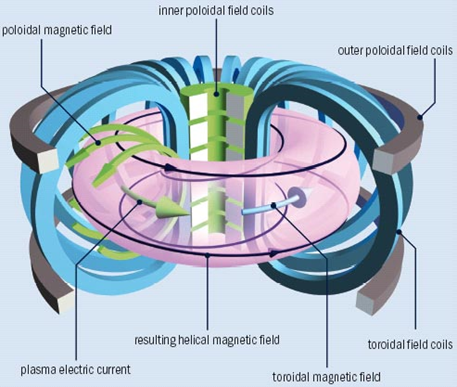
\includegraphics[width=1.2\columnwidth]{magAxis.png}
	\end{center}
	\end{figure}
\end{columns}
\end{frame}

\begin{frame}{Axisymmetric Configuration}{Poloidal Fluxes}
\begin{columns}
\column{0.4\textwidth}
	\begin{block}<1->{Magnetic Flux}
	   Mag. Poloidal flux (PF),  {\color<1->{blue}  $\Psi (R,Z) $} over one major
	   circle, at $(R, Z)$.

	    \color<1->{blue}
		{\small $ \begin{array}{rcl}
	    		\psi (R,Z) &=& \frac{\Psi (R,Z)}{ 2 \pi}    \textrm{ , \tiny flux per radian } \\
			\Psi (R,Z) &=& \iint \ d \vec{B} \cdot d  \vec{S}
	   		\end{array}$ }
	\end{block}
%   	\begin{figure}[ht]
	\pause
	\begin{center}
	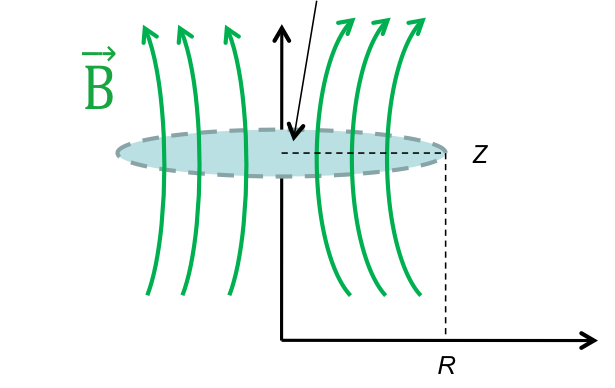
\includegraphics[height=2.5 cm ]{magflux.png}
	%\caption{\tiny }
	\end{center}
%	\end{figure}

\column{0.6\textwidth}

	\begin{block}<2->{Current Flux}
	%Current Flux
	  Poloidal current function, { \color<2>{red}  $F$},   crossing the major circle, at $(R,Z)$.
	    %\item
		\small
	    \color<2>{red} $ \begin{array}{rcl}
	    		F (R,Z) &=& \mu I_{pol} \Psi (R,Z) / 2 \pi  = R\, B_{\phi}  \\
			I_{pol}  (R,Z) &=& \iint \ d \vec{j}_{pol} \cdot d  \vec{S}
	   	\end{array} $
	  % \end{itemize}
	\end{block}
%  \end{cfx}

	\visible<2-> {\begin{center}
	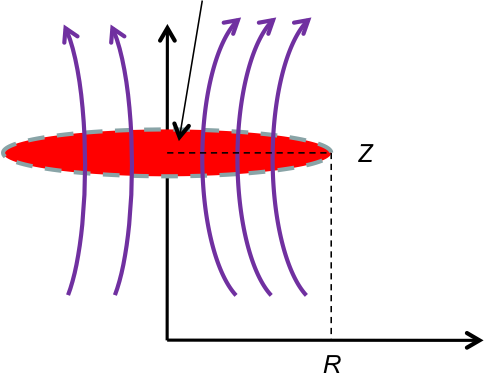
\includegraphics[height=2.5 cm]{currflux.png}
	\end{center}
	}

\end{columns}
\end{frame}

\begin{frame}{Axisymmetric Configuration}{Flux Surfaces}
Both Fluxes, { $\color{blue} (\Psi$}, {\color{red} $F$}) are constant on the  \texttt{Flux Surfaces}:
	\begin{figure}[ht]
	\begin{center}
	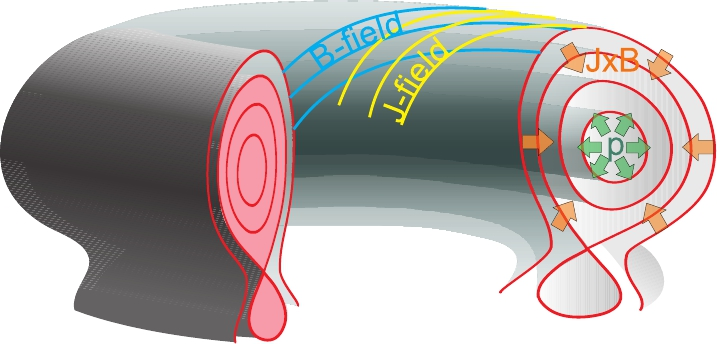
\includegraphics[width=.8\columnwidth]{Tokamak_Equilibrium.jpg} %{torfluxes.png}
	%\caption{\tiny The Astrolabe}
	\end{center}
	\end{figure}
\end{frame}


\begin{frame}{Toroidal Magnetic Field}
\begin{columns}
\column{0.6\textwidth}
\begin{block}<1->{Ampere$'$s Law}
$ \begin{array}{ccl}
   		\nabla \times \vec{B} &= & \vec{J_{free}} \\
%			//&= R B_{\phi}  \\
		\nabla F \times \hat{\phi} &=&  \mu_0 R \, J_{pol}   \textrm{ \small (poloidal comp.)}
  \end{array} $
\end{block}

   \begin{itemize}
   	\only<-2> {\item  \textbf{In vacuum:} $ \nabla F =0$, so $B_\phi (R)$ varies only  with $1 / R$
   	\begin{itemize}
   		\item  Result: No information from the plasma  taken from external local  $B_\phi $ measurements
 	\end{itemize}
	}
	\only<3->{\item \textbf{Within Plasma:} $B_\phi(R,Z)$ depends on poloidal currents, $J_{pol}$.
	    \begin{itemize}
   		\item \textbf{Diamagnetic loop} can measure the surface integral change.
	    \end{itemize}
	   }
   \end{itemize}

\column{0.4\textwidth}
%Both Fluxes, { $\color{blue} \Psi$}, {\color{red} $F$}   are constant on the  \texttt{Flux Surfaces}:
	\begin{center}
	%trim option's parameter order: left bottom right top
	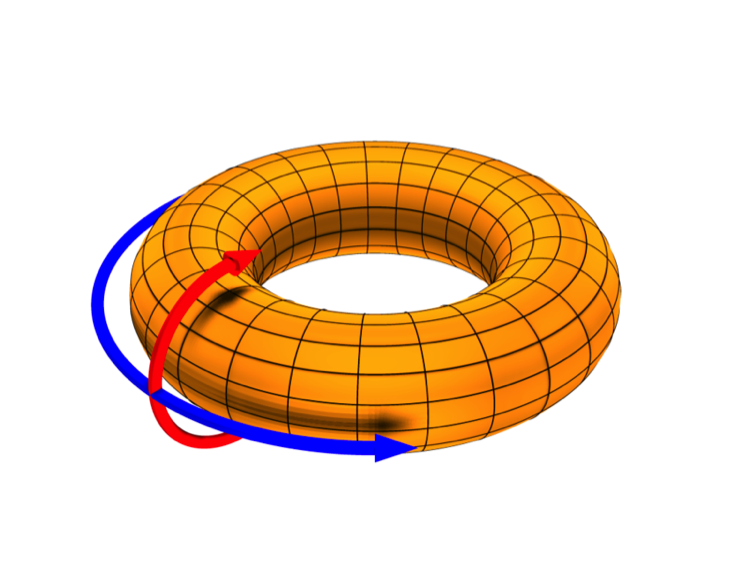
\includegraphics[trim = 2mm 5mm 2mm 5mm, clip, width=.7\columnwidth]{torsurf.png}
	$\color{blue} B_{\phi} = \frac{F}{R} $
	\includegraphics[width=.8\columnwidth]{btor.png}
	\end{center}
	\begin{tabular}{cc}
		\small	Diamagnetic & Paramagnetic
 	\end{tabular}
\end{columns}
\end{frame}

\begin{frame}{Poloidal Magnetic Field}
\begin{columns}
\column{0.5\textwidth}
\begin{block}<1->{Ampere$'$s Law { \small (toroidal comp.)}}
{ \small $ \Delta^* \Psi \equiv R \frac{\partial }{\partial R} (\frac{1}{R}  \frac{\partial \Psi }{\partial R} )  +
	\frac{\partial ^2 \Psi }{\partial Z^2}  = \mu_0 R \, J_\phi $  }
% { \small (toroidal comp.)}
\end{block}

%   \begin{itemize}
 %  	\item<2->
	$ \begin{array}{rl}
	  \Psi (x') &= - \int_\Omega G(x,x') J_\phi^{ext} (x) d x  \\
	  	&+ \oint_{\partial \Omega} \frac{1}{\mu_0 R} \left ( \Psi  \frac{\partial G }{\partial n}
		 - G \frac{\partial \Psi }{\partial n} \right ) dS \\
		x' &= \textrm{ \small point in } \Omega \\
		G(x,x')  &= \textrm{ \small  Green function for } \Delta^* \textrm{ \small operator.} \\
		 \frac{\partial  }{\partial n}   &= \textrm{ \small normal derivative}
		 %\\G(x,x') &=
	 \end{array} $
%   \end{itemize}

\column{0.5\textwidth}
	\begin{center}
		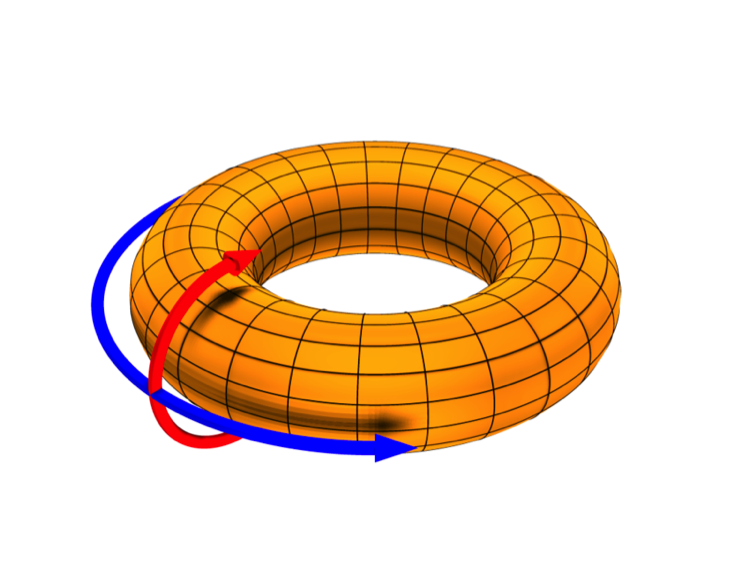
\includegraphics[width=.7\columnwidth]{torsurf.png}

		$\color{red} B_{p} = \frac{\nabla \Psi}{R} $

%	\end{center}
%	\begin{center}
		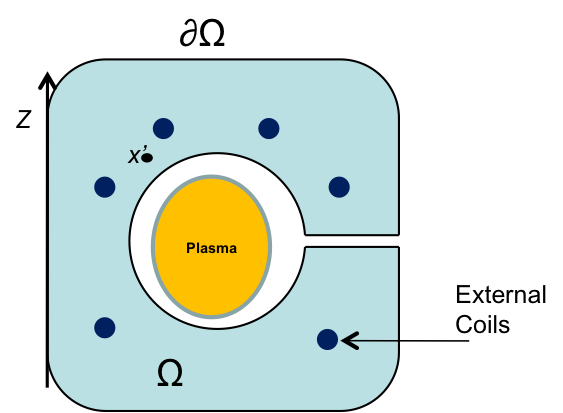
\includegraphics[width=.55\columnwidth]{xsection.png}
	\end{center}
\end{columns}
\end{frame}

 \begin{frame}{Equilibrium reconstruction}{Basic restriction for  the magnetic diagnostics }
 \begin{columns}
 \column{0.65\textwidth}
	\begin{block}{Green$'$s Theorem }
		$\Omega$ bounded by Plasma and $r \to \infty$.
	\end{block}

%	$ \begin{array}{rl}
%	  \Psi (x') &= - \int_\Omega G(x,x') J_\phi^{ext} (x) d x  \\
%	  	&+ \oint_{\partial \Omega} \frac{1}{\mu_0 R} \left ( \Psi  \frac{\partial G }{\partial n}
%		 - G \frac{\partial \Psi }{\partial n} \right ) dS \\
%		x' &= \textrm{ \small point in } \Omega \\
%		G(x,x')  &= \textrm{ \small  Green function for } \Delta ' \textrm{ \small oper.} \\
%		 \frac{\partial  }{\partial n}   &= \textrm{ \small normal derivative}
%		 %\\G(x,x') &=
%	 \end{array} $

$\Psi (x') = $

%	 \visible<2,3>  {\fbox{visible Text2}}
	\only<1>  { \fbox{ \color{blue}   $ - \int_\Omega G(x,x') J_\phi^{ext}(x) dx$, Currents in external coils }
			$ + \oint_{\partial \Omega} \frac{1}{\mu_0 R} \Psi  \frac{\partial G }{\partial n}  dS$ \\
			$  - \oint_{\partial \Omega} \frac{1}{\mu_0 R} G \frac{\partial \Psi }{\partial n} dS $
			}
	\only<2>  {   $ - \int_\Omega G(x,x') J_\phi (x) d x$\\
\fbox{ \color{red}  $ + \oint_{\partial \Omega} \frac{1}{\mu_0 R} \Psi  \frac{\partial G }{\partial n}  dS$ ,   $ \Psi = C^{nst}$  at the boundary } \\
			$  - \oint_{\partial \Omega} \frac{1}{\mu_0 R} G \frac{\partial \Psi }{\partial n} dS $}
	\only<3>  {   $ - \int_\Omega G(x,x') J_\phi (x) d x$\\
  			$ + \oint_{\partial \Omega} \frac{1}{\mu_0 R} \Psi  \frac{\partial G }{\partial n}  dS$ \\
\fbox{ \color{orange} $  - \oint_{\partial \Omega} \frac{1}{\mu_0 R} G \frac{\partial \Psi }{\partial n} dS $  }
			}

 \column{0.35\textwidth}
   \begin{center}
	%trim option's parameter order: left bottom right top
 	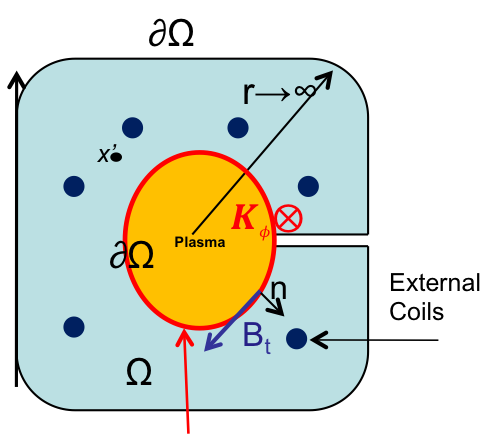
\includegraphics[trim = 1mm 1mm 8mm 1mm, clip, width=.7\columnwidth]{xsection2.png}

	{ \color{red}   $ \Psi = C^{nst}$  }
   \end{center}
 \end{columns}

 \visible<3->{ \begin{block}{}%$  - \oint_{\partial \Omega} \frac{1}{\mu_0 R} G \frac{\partial \Psi }{\partial n} dS $}
Term 3 is the only one that depends on internal current, $J_{\phi}^{plasma}$.
\end{block}
}
 \end{frame}

 \begin{frame}{Equilibrium reconstruction}{Basic restriction for  the magnetic diagnostics }
 \begin{block}{}
BUT solution depends only on $B_t$ distribution on the Plasma boundary.
Since many distributions, $J_\phi^{plasma}(r)$, give the SAME  $B_t$.
\end{block}

 \begin{block}{Reconstruction $\Psi(R,Z)$ in \textbf{Vacuum}  \smiley }
 {\color<1->{green}
		External  measurements can determine the $\Psi(R,Z)$ anywhere in $\Omega$  and  $B_t$  on
	$\partial  \Omega$. ~~~  \smiley
}
\end{block}

 \begin{block}{Reconstruction $\Psi(R,Z)$ inside  \textbf{Plasma} \frownie  }
%\fbox{
 {\color<2->{red}
	External  measurements alone  CANNOT distinguish  different internal current,
	$J_\phi(r)^{plasma}$ and $\Psi^{plasma}(R,Z)$ INSIDE the plasma! \frownie
}
%%}
\end{block}
\end{frame}

 \begin{frame}{Electrostatics Equivalent Parallel Case }
 The Electric Field outside the Sphere is the same for a given charge surface  density
or other (infinite) volume  distributions.
 \begin{columns}
 \column{0.5\textwidth}
	\begin{center}
	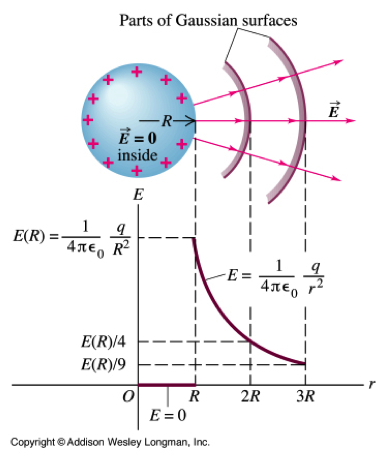
\includegraphics[width=.5\columnwidth]{surfcharge.png}
	\end{center}
 \column{0.5\textwidth}
	\begin{center}
	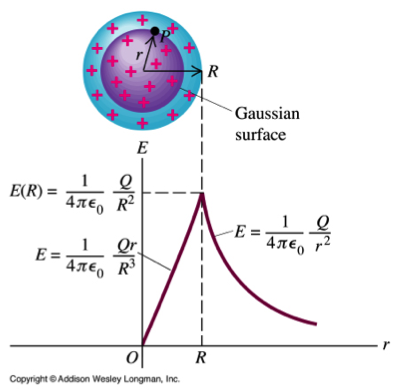
\includegraphics[width=.5\columnwidth]{volcharge.png}
	\end{center}

\end{columns}

 \begin{block}{Reconstruction inside a sphere }
	External  measurements  CANNOT distinguish different Volume charge distributions.
\end{block}
\end{frame}


\begin{frame}{Plasma Equilibrium in Fusion Plamas}{Grad-Shafranov Equation}
  \begin{itemize}
	 \item Combining equation for $\Psi$ with magnetic force balance  $\nabla p = \vec{J} \times \vec{B} $ gives “G-S”  equation inside the plasma: %“G-S”
		$$ \Delta^* \Psi = -\mu_0 R\, J_\phi=  -\mu_0 R^2  \frac{d p}{d \Psi} -  \frac{1}{2}  \frac{d F^2}{d \Psi}  $$
	\item G-S gives additional constraint on  $ \vec{B}$ within the plasma but also introduces another unknown scalar  functions:  the \alert{ pressure}  and \alert{current}
	\item Need to make some assumptions on $p(\Psi)$  and $F(\Psi)$ to calculate full plasma equilibrium “solution”.
  \end{itemize}

\end{frame}

\begin{frame}{Plasma Equilibrium}{Example: JET Reconstruction}
	\begin{figure}[ht]
	\begin{center}
		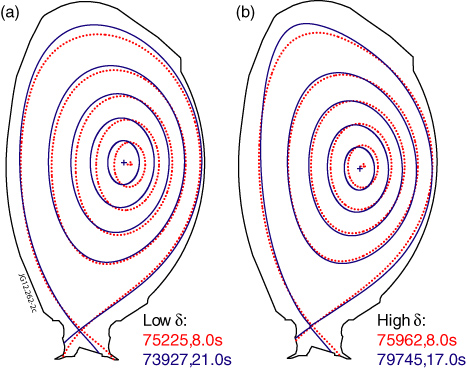
\includegraphics[width=.55\columnwidth]{JET_magFlux.jpg}
		\caption{\tiny  Magnetic configuration of the (a) low- and (b) high-triangularity plasmas for the hybrid (red) and baseline H-mode (blue) plasmas.}
	\end{center}
	\end{figure}
\end{frame}

\subsection{Global Inductive Magnetic Sensors }

\begin{frame}{Magnetic Inductive Sensors } {Basic Types}
	\begin{figure}[ht]
 	\begin{center}
	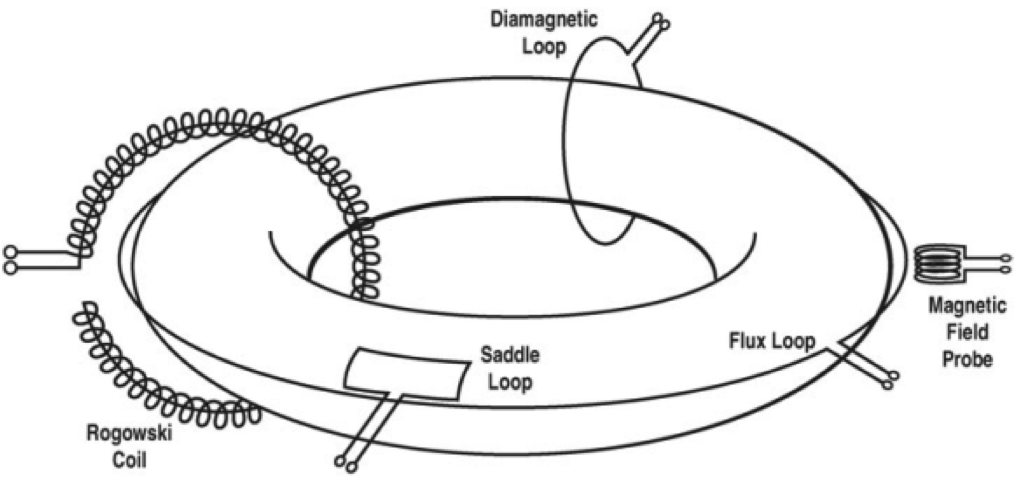
\includegraphics[height=3.5cm]{indsensors.png}
		\caption{\tiny Schematic figure of a toroidal plasma, showing the basic types of inductive sensors.}
	\end{center}
	\end{figure}
\end{frame}

\begin{frame}{Magnetic Inductive Sensors } {Signal is a time derivative }
% \begin{columns}
% \column{0.7\textwidth}
% \column{0.3\textwidth}
 	\begin{center}
 	\fbox{\parbox{0.5\textwidth}{
		Mag. Flux on the Sensor Loops }}
	%trim option's parameter order: left bottom right top
	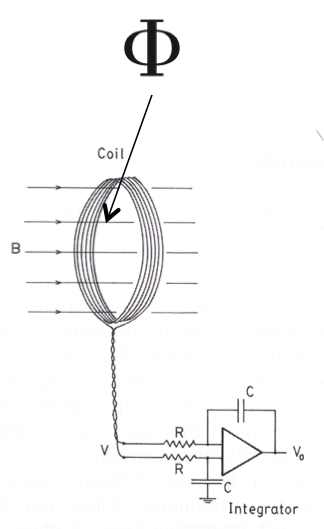
\includegraphics[trim = 1mm 25mm 3mm 5mm, clip, height=3cm]{magsensor.png}
	\end{center}
%\end{columns}
$
 \begin{array}{cl}
 V_{sensor} (t) &= \oint \vec{E} \cdot \vec{d s}  =
  - \frac{\partial \Phi(t)}{\partial t} = NA\dot {B}\textrm{ , Faraday Law} \\
\Phi(t) &= \int_{t_0}^t V(t') d t'
\end{array}
$

\end{frame}

\begin{frame}{Magnetic Inductive Sensors } {Rogowski Coil}

\begin{columns}
 \column{0.6\textwidth}
  \begin{itemize}
  \item Measures \alert{ total electric current} flowing through the enclosed surface,
	\begin{itemize}
	\item
		e.g. plasma, plasma + vessel, external coils, passive conductors, Halo Currents, etc.
	\end{itemize}
  \item   If $|\Delta B|/B \ll n $ ($n$ is turns / m),  total flux  is:
$\Phi = n \oint_\ell \int_A  \vec{B}\cdot  \vec{d \ell} d A = n A \mu_0 I_p$
\item Signal is proportional to current time derivative: $ V(t)= \dot{\Phi} =  n A \mu_0 \dot{I_p}$
	\end{itemize}
 \column{0.4\textwidth}
	\begin{center}
	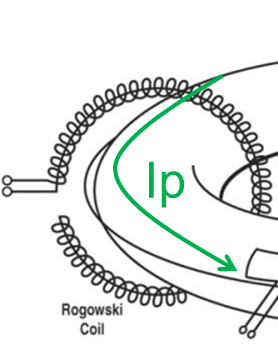
\includegraphics[width=.7\columnwidth]{rogow.png}
	 \begin{block}{}
		\small Conducting path from one end must return along the axis to the other end
	\end{block}
	\end{center}

\end{columns}
\end{frame}

\begin{frame}{Magnetic Inductive Sensors } {Sinus-cosinus Coil}

\begin{columns}
 \column{0.6\textwidth}
  \begin{itemize}
  \item A variation of Rogowski Coil but winding density, $n(\theta)$, varies with $ \sin (\theta) $ or $ \cos (\theta) $
  \item Used to measure Plasma Displacements	\arrowright
\end{itemize}
 \column{0.4\textwidth}
	\begin{center}
	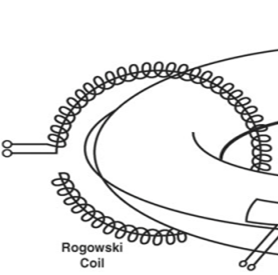
\includegraphics[width=.9\columnwidth]{sinus.png}
	\end{center}

\end{columns}
\end{frame}

\begin{frame}{Magnetic Inductive Sensors } {Poloidal Flux  Loops}
\begin{columns}
 \column{0.6\textwidth}
  \begin{itemize}
  \item Measures $\Psi(R, Z)$ on a given $(R, Z)$
  \item On Iron Core Tokamaks with ohmic heating, most of the poloidal flux is on the core itself:
$B = \mu_r \mu_0 H, \, \mu_r(iron) \approx 4000$
 \item To improve the sensivity, a smaller loop is chosen as reference and subtracted from others:
$\Psi_{i} =\Psi(R, Z)  - \Psi_{ref} $
 \end{itemize}

 \column{0.4\textwidth}
	\begin{center}
	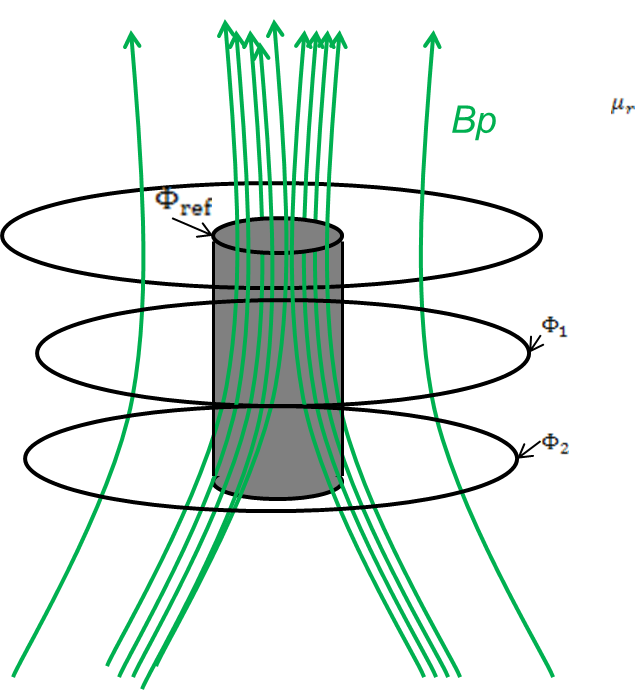
\includegraphics[width=.6\columnwidth]{fluxloops.png}
   	\begin{block}{Loop Voltage}
		Voltage signal from a flux loop is the local one-turn
	$V_{loop}$, which drives $I_p$
  	\end{block}
	\end{center}

\end{columns}
\end{frame}

\begin{frame}{Magnetic Inductive Sensors } {Diamagnetic Loop}
\begin{columns}
 \column{0.5\textwidth}
     \begin{itemize}
	 \item Measure the toroidal magnetic flux for the purpose of estimating the thermal energy of the plasma $\langle p \rangle  \propto W$.
	 \item Normally located in a poloidal plane  to minimize coupling to the $B_{pol}$.
	\item At low beta, the change in the total toroidal flux is small.
	$\beta = 2 \mu_0 \langle p \rangle  /B^2 \ll 1$
     \end{itemize}
 \column{0.5\textwidth}
	\begin{center}
	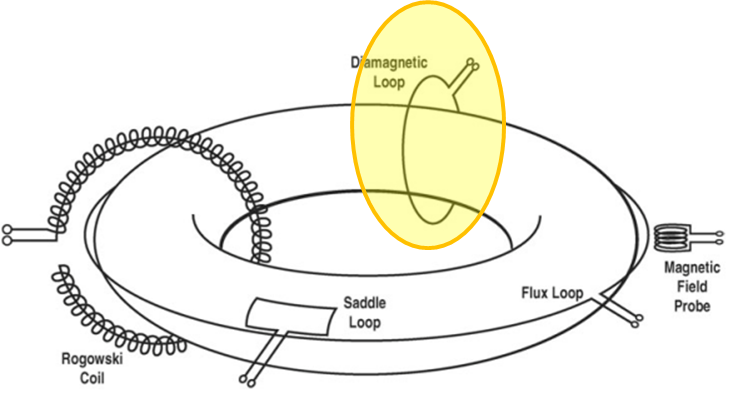
\includegraphics[width=1.0\columnwidth]{diamag.png}
	 \begin{block}{}
		 A reference signal coupled to $B_{\phi, vacuum}$ is usually subtracted:
		$ \Delta \Phi_{Diag} =  \Phi_{total}  -   \Phi_{vacuum}$ % \approx \frac{2 \kappa}{1 +\kappa^2}  \frac{(\mu_0 I_p)^2}{8 \pi B_{\phi, vacuum)}} (1 - \beta_p) $
	\end{block}
	\end{center}

\end{columns}
\end{frame}

\subsection{Plasma Integral  quantities }

\begin{frame}{Basic Magnetic Inductive Sensors } { Integral  quantities}
   \begin{itemize}
 	\item Total \textbf{ Plasma Current }, $I_\phi$  ( Rogow.)
	\item  \textbf{ Ohmic Power}  ( Rogow+ V. Loop)
	$$P \equiv \int_{Vol} \vec{E} \cdot \vec{j}\, d^3 x = V_\phi I_\phi - \frac{\partial}{\partial t} (\frac{1}{2} L I_\phi^2 ) $$

	\item \textbf{ Poloidal beta }, $\beta_p $,  ( Rogow+ Diag. Lop)
	 $	\beta_p \equiv 2 \mu_0 \langle p \rangle  / B_{p,a}^2 ( \ll 1)$ , $B_{p,a} = \mu_0\, I_\phi / \Gamma $,  $ \Gamma$ is length of a poloidal plasma contour.
   	\begin{itemize}
 		\item Circular Plasma $  \beta_p = 1 - \frac{8 \pi B_{\phi, vacuum}}{(\mu_0 I_\phi)^2} \, \Delta \Phi_{Diag} $
	 	\item Non-Circular Plasma
		$$  \beta_p  \approx  1  - \frac{1 +\kappa^2}{2 \kappa}  \frac{8 \pi B_{\phi, vacuum}}{(\mu_0 I_\phi)^2} \, \Delta \Phi_{Diag}$$
		$\kappa$ is the vertical elongation of plasma
	    \end{itemize}
     \end{itemize}
%	Proportional to \textbf{ Plasma thermal energy}
\end{frame}


\begin{frame}{Basic Magnetic Inductive Sensors } {Integral  quantities II}
   \begin{itemize}
 	\item Total \textbf{“Shafranov shift” }, $\Delta$.  ( From Rogow. + Vertical Field Current)
     \end{itemize} At Large Aspect Ration approximation:

$$\Delta' = \frac{r}{R} \Lambda, \quad \Lambda=\beta_{pol} + \ell_i /2$$
	\begin{center}
   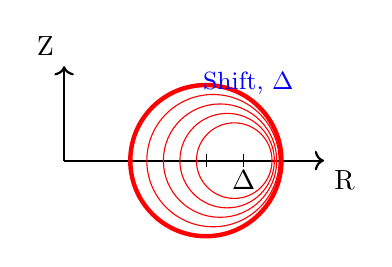
\begin{tikzpicture}[scale=0.6]
	\draw [thick,->]  (-3,0) -- (2.5,0) node[anchor=north west] {R};
	\draw [thick,->] (-3,0) -- (-3,2)  node[anchor=south east] {Z};
	\draw [red] (0.6, 0) circle [radius=0.8];
	\draw [red] (0.45, 0) circle [radius=1.0];
	\draw [red] 		 (0.3, 0) circle [radius=1.2];
	\draw [red] 		 (0.15, 0) circle [radius=1.4];
	\draw [red, ultra thick] (0.0, 0) circle [radius=1.6];
	\node[blue, align=center, above] at (0.9,1.2) {\small Shift, $\Delta$};
	\draw [|-|] (0,0) -- (0.8,0)  node[anchor=north] {$\Delta$};
  \end{tikzpicture}
	\end{center}
\end{frame}
%		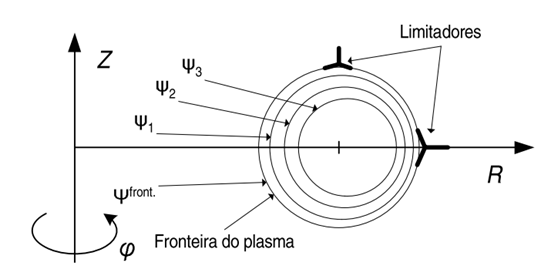
\includegraphics[width=.75\columnwidth]{shafran.png}

\begin{frame}{Basic Magnetic Inductive Sensors } {Integral  quantities III}
   \begin{itemize}
	\item \textbf{ Plasma conductivity }, $\sigma$ ( Rogow+ V. Loop)
		$$ \hat{\sigma} =\frac{2 \pi\, R}{\pi a^2} \frac{I_\phi^2}{P}, (\textrm{ if } \frac{\partial}{\partial t} =0 ) $$
   	\item  \textbf{Electron Temperature }, $T_e$
	$$ \sigma = 1.9 \times 10^4 \left (\frac{T_e^{3/2}}{Z_\sigma \ln \Lambda } \right )  $$
	\begin{itemize}
		\item  $Z_\sigma$, resistance anomaly determined by ion charge
		\item  $\ln \Lambda  $, Coulomb logarithm:
		$$ \ln \Lambda  \approx 31 - \ln(n_e^{1/2} / T_e)$$
	\end{itemize}

     \end{itemize}
\end{frame}

\begin{frame}{Magnetic Inductive Sensors } {Plasma Displacement}
\begin{columns}
 \column{0.5\textwidth}
   \begin{itemize}
 	\item Cylindrical Approximation $R \gg a$. Plasma Displaced by $ \Delta \ll a$
    \end{itemize}
 \column{0.5\textwidth}

   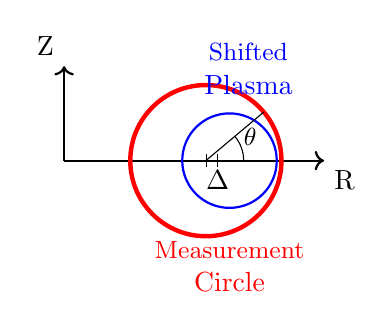
\begin{tikzpicture}[scale=0.6]
	\draw [thick,->]  (-3,0) -- (2.5,0) node[anchor=north west] {R};
	\draw [thick,->] (-3,0) -- (-3,2)  node[anchor=south east] {Z};
	\draw [blue,  thick] (0.5, 0) circle [radius=1.0];
	\draw [red, ultra thick] (0.0, 0) circle [radius=1.6];
	\draw  (.8,0) arc [radius=0.8, start angle=0, end angle= 40]; 			%[gray]
	\draw [rotate=40] (0,0) -- (1.6,0) ;
	\node[blue, align=center, above] at (0.9,1.2) {\small Shifted \\ Plasma};
	\node[red, align=center, below]  at (0.5,-1.5) {\small Measurement \\  Circle};
%	\draw [| ] (0,0) -- (0.5,0)  node[anchor=north] {$\Delta$};
	\draw [|-|] (0,0) -- (0.25,0)  node[anchor=north] {$\Delta$};
	%\node[below]  at (0.25,0.0) {$\Delta$};
	\node[right]  at (0.6,0.5) {\small $\theta$};
%
%	\draw [thick] (0,1.5) -- (3,0);
%	\draw [ultra thick] (0,0) -- (2,2);
%	\draw [help lines] (1,0) -- (1,1) -- (0,1);
  \end{tikzpicture}
  \end{columns}
   \begin{itemize}
	\item Measured poloidal field is:
	$$ \begin{array}{rcl}
		B_\theta (\theta) &=& \frac{\mu_0 I}{2 \pi a} \frac{1}{\left [ \sin^2 \theta + (\cos \theta - \Delta/a)^2 \right ]^{1/2}} \\
				    &=&\frac{\mu_0 I}{2 \pi a} \left (   1 + \frac{\Delta}{a} \cos \theta \right )
	\end{array}  $$
	\item Displacement can extracted from the Sinus-cosinus Coils: $\Delta = 2 a (C_1/C_0) $.
    \end{itemize}
\end{frame}


%%%%%%%%%%%%%%%%%%%%%%%%%%%%%%%%%%%%%%%%%%%%%%
\subsection{Local Inductive Magnetic Probes }

\begin{frame}{Magnetic Probes} % { Integral  quantities II}
\begin{columns}
 \column{0.6\textwidth}
     	\begin{itemize}
		\item Probes measure components of the local magnetic field strength.
		\item Usually solenoidal, with dimensions small compared to the gradient scale length of the magnetic field.
	\end{itemize}
 \column{0.6\textwidth}
	\begin{center}
	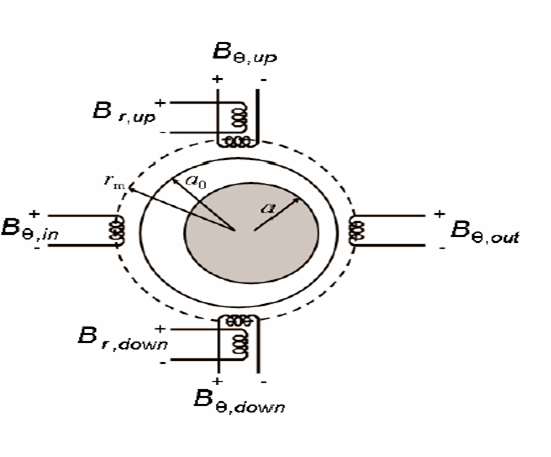
\includegraphics[width=.6\columnwidth]{magProbes.png}
	$$\Phi_{probe} = N\, A\, B_{\parallel}$$
	\end{center}

\end{columns}
\end{frame}

\begin{frame}{Magnetic Local Probes}{Shielding}
\begin{columns}
 \column{0.65\textwidth}
     	\begin{itemize}
		 \only<1>{\item Probes should be located on the plasma-facing side of the vacuum vessel wall.}
		\item
		 \only<1>{ Should be oriented to measure the field tangential to the wall; otherwise, eddy currents in the wall will attenuate the high-frequency part of the signal.}
		 \only<2>{ Shielding of the tangential field by the conductive wall.
		                              $$\begin{array}{rcl}
			  \frac{B_{\par}(inside) }{B_{\par 0}} &=&  \frac{1 + 2 i \omega \tau_w }{1 +  i \omega \tau_w}\\
			 \frac{B_{\par}(outside) }{B_{\par 0}} &=&  \frac{1  }{1 +  i \omega \tau_w}
		     \end{array}$$  $ \tau_w$ is the characteristic time for the magnetic flux to diffuse through the wall  }
		\end{itemize}
 \column{0.35\textwidth}
	\begin{center}
	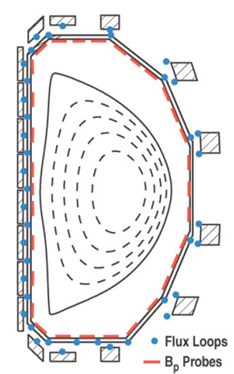
\includegraphics[width=0.7\columnwidth]{probeShield.png}
	\end{center}

\end{columns}
\end{frame}

\begin{frame}{Saddle Loops}%{Shielding}
\begin{columns}
 \column{0.6\textwidth}
	Can be viewed as
     	\begin{itemize}
		\item  A large-scale magnetic probe for the magnetic field normal to the surface. $\Phi(saddle) = N \, A \langle B_{\perp} \rangle $
		\item or as probes measuring Flux Difference: . $\Phi(saddle) = N \,  \Delta_\phi \,  \Delta_\psi $
	\end{itemize}
 \column{0.6\textwidth}
	\begin{center}
	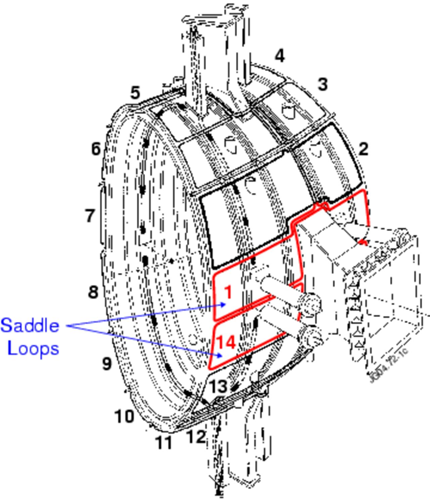
\includegraphics[width=0.6\columnwidth]{Saddle.png}
	\end{center}

\end{columns}
\end{frame}

\subsection{Plasma Shape }

\begin{frame}{Determination of Plasma Shape }%{}
   	\begin{enumerate}
		\item Taking measurements of the $\Psi(R,Z)$ and poloidal $B_{pol}$ near the Wall, plus the currents in external Coils allows
			local $\Psi$ extrapolation.
		\item<2-> Plot the contours of $\Psi(R,Z)=C^{nst}$. Find the Last Closed Flux Surface {\color{red} LCFS}, or  {\color{blue} Separatrix} in Divertor tokamaks
	\end{enumerate}
\begin{columns}
 \column{0.6\textwidth}
     \begin{tikzpicture}[scale=0.4]
	\node [below left] at (0,0)   {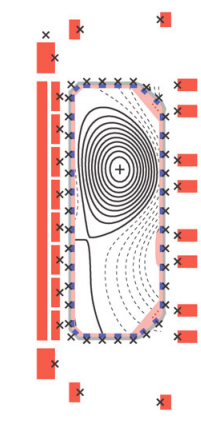
\includegraphics[height=4 cm]{LCFS.png}};
	\draw [thick,<-]  (-3,-1) -- (0.5,-1) node[anchor= west]{Flux Loops $\Psi(R,Z)$};
	\draw [red, thick,<-]  (-1.8,-3.5) -- (0.5,-3.5) node[red, anchor= west]{LCFS};
	\draw [thick,<-]  (-1.3,-5.6) -- (0.5,-5.6) node[anchor= west]{Magnetic Probes $B(R,Z)$};
%	\draw [thick,<-]  (0,0) -- (1,0) node[anchor=north west] {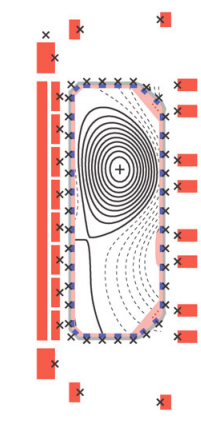
\includegraphics[width=0.2\columnwidth]{LCFS.png}};
%	\draw [thick,->] (-3,0) -- (-3,2)  node[anchor=south east] {Z};
     \end{tikzpicture}
%
  \column{0.6\textwidth}
	\begin{center}
	     \begin{tikzpicture}[scale=0.4]
		\node [above right] at (0,0)   {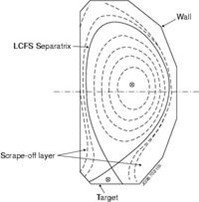
\includegraphics[height=3 cm]{Separatrix.png}};
		\draw [blue, thick,<-]  (3.2,3) -- (1,3) node[blue, anchor= east]{Separatrix};
	     \end{tikzpicture}
	\end{center}
\end{columns}
\end{frame}

%%%%%%%%%%%%%%%%%%%%%%%%%%%%%%%%%%
\section{Integration of signals from inductive sensors}

\begin{frame}{Integration of signals from Mag. Sensors}{Analog Integration}
   	\begin{itemize}
	    \item To obtain the fluxes and magnetic field values from inductive sensors we must integrate the signal in time:
$V_{out}(t) = -\frac{1}{\tau} \int_0^t V_{in}(t') dt' = \Phi (t)  / \tau $

	\begin{center}
	     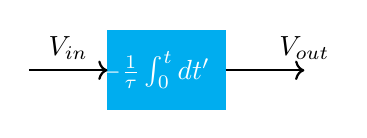
\begin{tikzpicture}[scale=0.5]
		\draw [fill=blue, cyan] (2,0) rectangle (5,2) ;
		\node[white] at (3.2,1) {$ -\frac{1}{\tau} \int_0^t dt'$};
%		\draw [fill=blue, cyan] (2,0) rectangle (4,2)
%		node[white]{ $ -\frac{1}{\tau} \int_0^t $};
%		\draw [fill=blue, cyan] (2,0) rectangle (4,2)  node[white, below right]{ $ -\frac{1}{\tau} \int_0^t $};
		\draw [thick]  (0,1) -- (1,1) node[above ]{ $V_{in}$};
		\draw [thick,->]  (1,1) -- (2,1);	% node[above ]{ $V_{in}$};
		\draw [thick,->]  (5,1) -- (7, 1) node[above ]{ $V_{out}$};

    	 \end{tikzpicture}
       \end{center}
	\item Typical loop flux values vary from few $mV.s$ to $V.s$ (e.g. Iron core), so integrator circuits are used with  $1\,ms < \tau < 1\,s$.
     \end{itemize}
\end{frame}

\subsection{Analog Integration}
\begin{frame}{Integration of signals }{Analog Passive Integrator}
	\begin{center}
	%
	\ctikzset{bipoles/length=.8cm}
	\begin{circuitikz}[scale=0.5, transform shape]
	    \draw (0,2) node[anchor=east]{$V_i$}
		%to [short , o-] (1,2)
	    	to [R, l =$R$, o-] (2,2) % R=1<\ohm>] (2,2)
	    	to [short ,*-o] (4,2)  node[anchor=west]{$V_o$}
	        	(0,0) to [short , o-*] (2,0)
	    	to [C=1<\farad>] (2,2)
	    	(2,0) to [short ,*-o] (4, 0) ;
	\end{circuitikz}
	\end{center}
   	\begin{itemize}
		\item Simple Passive Integrator (RC Low Pass Filter, $1^{rst}$  Order , $-20dB/dec$.), $ \tau =RC$
		$$  V_{out}(\omega) =  -\frac{1}{1+i \omega \tau} V_{in}(\omega) \Rightarrow V_{out}(t)
		 \approx  -\frac{1}{\tau} \int_{t_0}^t  V_{in}(t') dt' $$
	\only<1->{
		\begin{block}{RC Limitation! }
			The approximation fails for timescales $ t \geq RC$.
		\end{block}
	}
	\end{itemize}
\end{frame}

\begin{frame}{Integration of signals }{Analog Active (Op-Amp) Integrator}
\begin{columns}
 \column{0.5\textwidth}
	\begin{itemize}
		\item Gain is similar to passive integrator, $1/RC$, but timescale is increased  from $\sim RC \to \sim G \cdot RC$ ~~~~ ($1\,ms$ to $10\,s$).
	\end{itemize}
%	    \alert<2->
%	\only<2>{
%		\begin{block}{Integrator Drift }
%			But now a NEW  problem:
%			Example: for $RC = 10\,ms$ a $V_{off}=100\,\mu V$ integrates to a $0.1 V$ after $10 s$
%		\end{block}
%	}

  \column{0.5\textwidth}
    \begin{center}
	\only<1>{
		\begin{block}{ NEW  problem: Integrator Drift by OpAmp Input $V_{off}$  }
			Example: for $RC = 10\,ms$ a $V_{off}=100\,\mu V$ integrates to a $0.1 V$ after $10 s$
		\end{block}
	}
	%
%	\only<1>{\begin{block}{Solution} Basic compensation circuit \end{block}}
	\ctikzset{ bipoles/thickness=2}
	\begin{circuitikz}[scale=0.5, transform shape]
	   \draw
	   (5,.5) node[op amp] (opamp) {G}
	   (0,1) node[left ]{$V_{in+}$} to [R, l =$R$, o-*] (2.5,1) to (opamp.-)
	   (opamp.out) |- (4.5,2) to [C, l_=$C$] (3.5,2) -- (2.5,2) to [short] (2.5,1)
	   (opamp.out) to [short , *-o] (7,.5) node[ right ]{$V_{out}$}
	  (opamp.-)  to [open, v<=$v_{off}$, color=red] (opamp.+)
	   (0,0) node[left ]{$V_{in-}$} to [R, l =$R$] (2.5,0) to (opamp.+) to  [C, l_=$C$, *-] ($(opamp.+)+(0,-2)$)   node[ground] {} ;
%
%	   \uncover<2>{\draw[color=red]  (6,2) |-  (4.5,4) to [generic, l=$Feedback$] (3.5,4)  -- (2.5,4) to [short] (2.5,1);}
	   \only<2>{\draw[color=red]  (6,2) |-  (4.5,4) to [generic, l=$Feedback$] (3.5,4)  -- (2.5,4) to [short] (2.5,1);}
	\end{circuitikz}
%
	\only<2>{\begin{block}{Solution} Basic compensation circuit \end{block}}
  \end{center}
\end{columns}
\end{frame}

\begin{frame}{Analog Integrators}{Advanced Designs}
\begin{columns}
  \column{0.5\textwidth}
	\begin{itemize}
		\item Automatic drift-compensation: Measurement of drift before integration, store and compensate offset during integration.
		\item<2-> Drift can be reduced down to  several $0.1mVs @ 1000s$
		\item<3->  But worse values if signal  is applied during drift  compensation!
	\end{itemize}
\column{0.5\textwidth}
	\begin{center}
	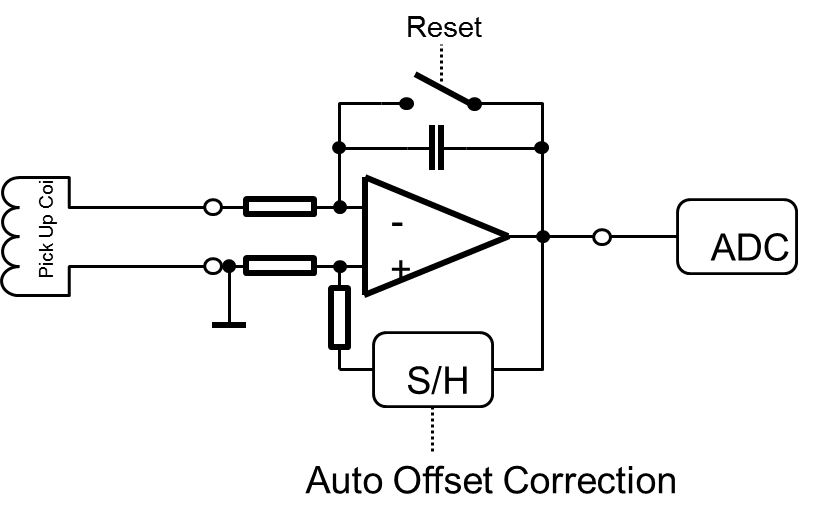
\includegraphics[width=0.8\columnwidth]{toreSupreInt.png}
	\begin{block}<4->{Tore Supra}
	Drift achieved: $ < 135 \mu Vs @ 1000\,  s$

%		 %		 A reference signal coupled to $B_{\phi, vacuum}$ is usually subtracted:
%		$ \Delta \Phi_{diag} =  \Phi_{total}  -   \Phi_{vacuum}$ % \approx \frac{2 \kappa}{1 +\kappa^2}  \frac{(\mu_0 I_p)^2}{8 \pi B_{\phi, vacuum)}} (1 - \beta_p) $
	\end{block}
	\end{center}
\end{columns}
\end{frame}

%%%%%%%%%%%%%%%%%%%%%%%%%%
\subsection{Digital Integration}
\begin{frame}{Digital Integrators}{Chopper Input}
	\begin{center}
		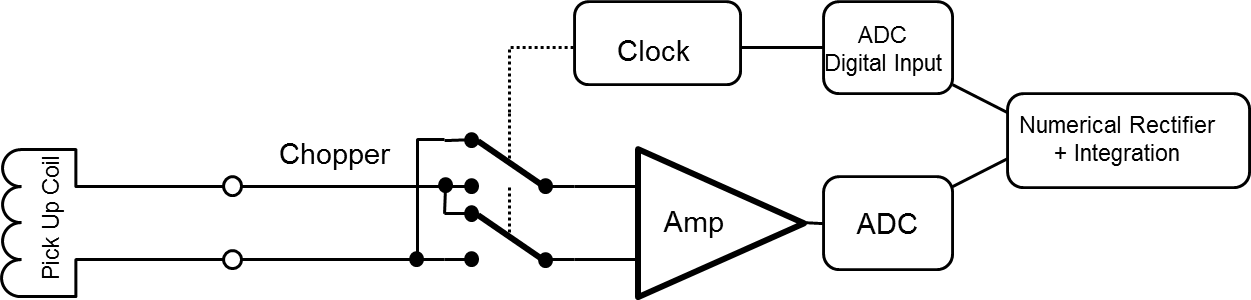
\includegraphics[width=0.8\columnwidth]{chopperInt.png}
	\end{center}
	\begin{itemize}
		\item Dynamic range limited by input stage
		\item Not affected by input stage semiconductors
%		\tem  No $1 / f$ noise
		\item Complex offset correction algorithms feasible
%\ Very simple consumer electronics!
 	\end{itemize}
%
%\begin{columns}
%
%\end{columns}
\end{frame}

\begin{frame}{Digital Integrators}{W7-X / IST ADC chopper module}
	\begin{center}
		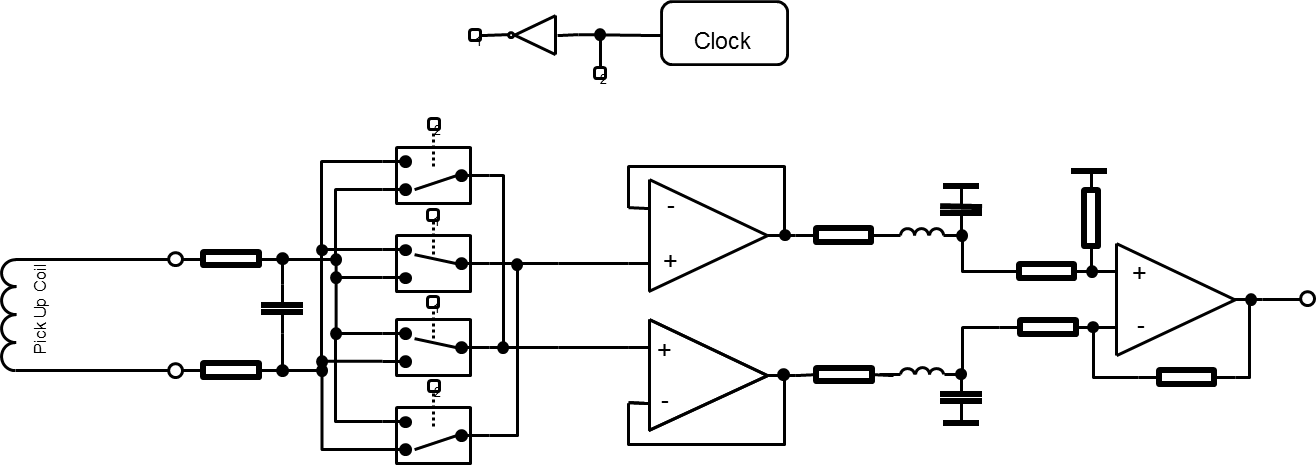
\includegraphics[width=0.7\columnwidth]{w7xSchema.png}

		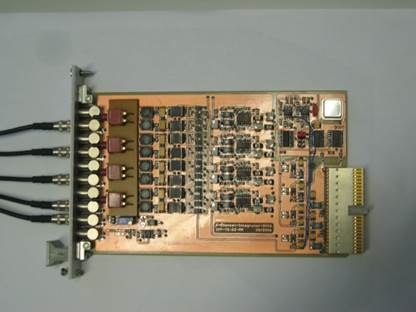
\includegraphics[height = 3 cm]{w7xInt.jpg}
	\end{center}
\end{frame}

\begin{frame}{Digital Integrators}{IST prototype}
\begin{columns}
  \column{0.3\textwidth}
	\begin{itemize}
		\item $100 s$ drift  compensation
		\item $1000 s$ run “Cold Integrator”
	\end{itemize}
    \column{0.7\textwidth}
	\begin{center}
		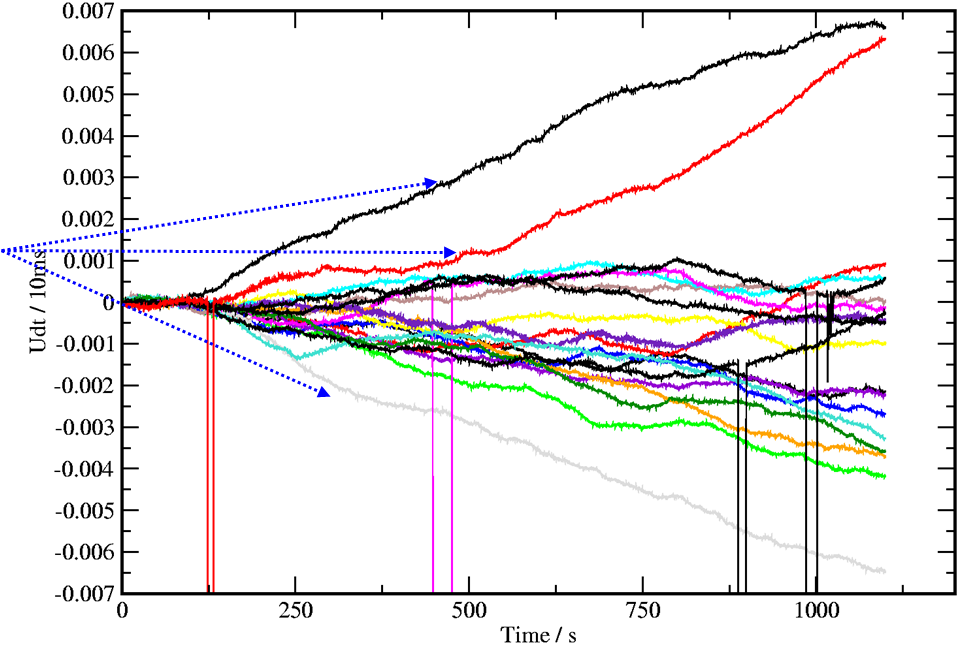
\includegraphics[height = 3 cm]{w7xDrift.png}

		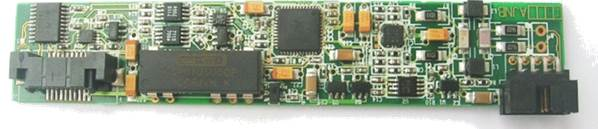
\includegraphics[height = 1 cm]{AtcaAdc.jpg}
	\end{center}
\end{columns}
\end{frame}



%%%%%%%%%%%%%%%%%%%%%%%%%%
\section{Non-Integrated signals}

%non-Integrated signal from Inductive probes
\subsection{Non-Integrated signals}
\begin{frame}{Non-Integrated Signal}{Inductive probes}
\begin{columns}
  \column{0.4\textwidth}
	\begin{itemize}
		\only<1> { \item Usally as linear combinations of flux Loop and/or field probes ( analog adders)
			        \item Direct information on Plasma Speed:  $V(t) \propto Vel_{R,Z}(t)$
			\begin{itemize}
				\item Used as controllable variables for active control
			\end{itemize}
 		}
		\only<2> {\item High Frequency MHD plasma instabilities  detection and control $V(t) \propto \dot{B(t)}  \sim \omega B(t)$
			\begin{itemize}
%				\item MHD instabilities detection and control
				\item “Mirnov coils”, poloidal or toroidal arrays  oriented to measure $\dot{B_{pol}}(t) $%, inside the vacuum vessel
			\end{itemize}
		}
	\end{itemize}

  \column{0.6\textwidth}
	\begin{center}
		%trim option's parameter order: left bottom right top
		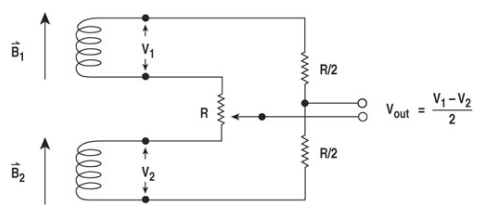
\includegraphics[trim = 0mm 0mm 0mm 1mm, clip, height = 2cm]{probesSum.png}

		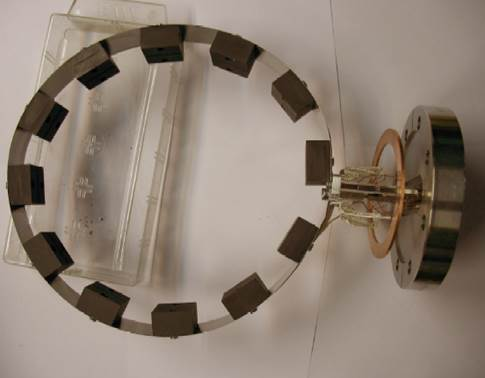
\includegraphics[height = 2.cm]{isttokMirn.jpg}
	\end{center}
\end{columns}
\end{frame}

\subsection{MHD Instabilities Diagnostics}
\begin{frame}{Non-Integrated Signal}{MHD Instabilities Diagnostics}
	\begin{itemize}
		\item Analyses Techniques: Spectrogram (Fourier analysis of successive short-time windows).
		\item Other techniques:
		\begin{itemize}
			\item Wavelet  analysis.
			\item Hilbert transform.
			\item Singular Value Decomposition (SVD).
		\end{itemize}
	\end{itemize}
	\begin{figure}[ht]
		\begin{center}
			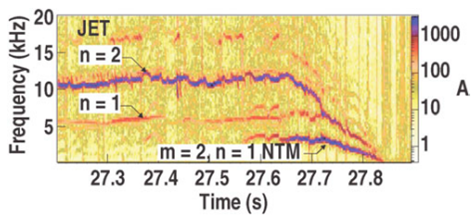
\includegraphics[width=0.6 \columnwidth]{SpectrogramJET.png}
			\caption{\small Spectrogram of magnetic probe signals in JET, showing the time evolution of the amplitudes and frequencies of several tearing modes.}
		\end{center}
	\end{figure}
\end{frame}

\begin{frame}{Non-Integrated Signal}{MHD Instabilities mode number detection}
 \begin{itemize}
	\item Usual MHD perturbation: $\delta B(t) \propto \delta B(r) \cos (m\theta + n\phi -\omega t ) $
		 \item Mode numbers {\color{red}  $m, n$}  are determined by the phase shift between equally separated Mirnov coils, by Fourier Analysis.
% %		\item Other techniques:
	 \end{itemize}
	 \begin{columns}
  	     \column{0.5\textwidth}
		% \begin{figure}[ht]
			% \begin{center}
				% 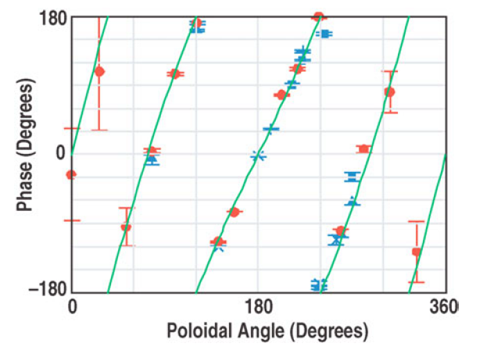
\includegraphics[width=0.7 \columnwidth]{TFTR.png}
				% \caption{\tiny Identification of poloidal mode number {\color{red}  $m=4$} for a tearing mode in TFTR	.}
			% \end{center}
		% \end{figure}
  	    % \column{0.5\textwidth}
		 \begin{figure}[ht]
			 \begin{center}
				 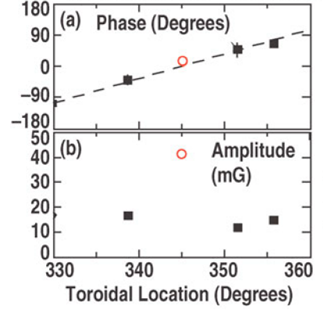
\includegraphics[width=0.4 \columnwidth]{NSTX.png}
				 \caption{\tiny Identification of the toroidal mode number {\color{red}  $n=7$} of a compressional Alfven eigenmode in NSTX.}
			 \end{center}
		 \end{figure}
 	  \end{columns}
% %
% %
\end{frame}


\begin{frame}{Non-Integrated Signal}{Auto and Cross Correlation between two signals}
Defining a dot product between 2 functions…
$$<f,g>= \int_{-\infty}^{\infty} f^*(t) g(t) dt$$
Cross-correlation :
$$ \begin{cases}  (f \ast g) (\tau)= \int_{-\infty}^{\infty} f^*(t) f(t +\tau) dt & \text{Continuous,}\\
 (f \ast g) [n]= \sum_{m=-\infty}^{\infty} f^*[n] g[n+m]  & \text{Discrete.} \end{cases} $$

Auto-correlation :
 $$ \begin{cases} (f \ast f) (\tau)= \int_{-\infty}^{\infty} f^*(t) f(t +\tau) dt & \text{Continuous, }\\
 (f \ast f) [n]= \sum_{m=-\infty}^{\infty} f^*[n] f[n+m]  & \text{Discrete.} \end{cases} $$
\end{frame}

\begin{frame}{Non-Integrated Signal}{Auto and Cross Correlation between two signals}
Cross-correlation of “real life” finite sampled signals
\begin{itemize}
\item Real life signals have only limited number of samples
\item Cross-correlation easier to interpret when bounded in [-1,1]
\item Lag vector (index-n) also finite
\item MATLAB/Octave Funtion \emph{r= xcorr( x , y )}
\end{itemize}

$$(f \ast g) [n]=  \begin{cases}
      \frac{\sum_{m=1}^{N-|n|} (f[m +|n|] - \bar{f} ) (g[n] - \bar{g} ) } {\sqrt{\sum_{m=1}^{N} (f[m] - \bar{f})^2}\sqrt{\sum_{m=1}^{N} (g[m] - \bar{g})^2}}& \text{if } n < 0,\\
\\
      \frac{\sum_{m=1}^{N-n} (f[m] - \bar{f} ) (g[n+m] - \bar{g} )} {\sqrt{\sum_{m=1}^{N} (f[m] - \bar{f})^2}\sqrt{\sum_{m=1}^{N} (g[m] - \bar{g})^2}} & \text{if } n \ge 0.
    \end{cases}$$

\end{frame}

\begin{frame}{Non-Integrated Signal}{Cross Correlation as wavenumber  \emph{m, n} estimator}
\begin{columns}
\column{0.6\textwidth}
{ $ \begin{array}{rcl}
	    		f[n]  &=&  \cos(w_1 t[n ] - k \theta_1 )   \\
			g[n]  &=& \cos(w_1 t[n ] - k \theta_2 ) \\
	   		\end{array}$ }
\~
{ $ \begin{array}{rcl}
	    		w_1 t[n + lag_{max}] - k \theta_2 &=& w_1 t[n ] - k \theta_1    \\
			w_1 (t[n + lag_{max}] -  t[n ])   &=& k ( \theta_2 -\theta_1) \\
			k  &=& \frac{w_1 \cdot t[lag_{max}]}{ \theta_2 -\theta_1}
	   \end{array}$ }
\column{0.4\textwidth}
	\begin{center}
	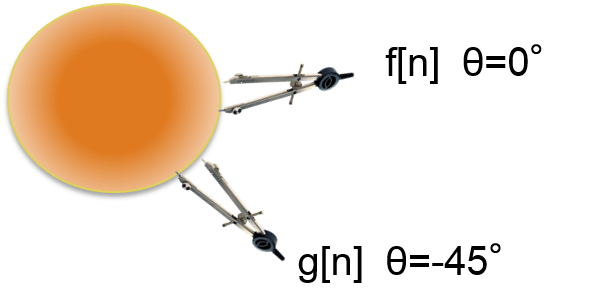
\includegraphics[width=0.9 \columnwidth]{figures/k-wave.png}
	\end{center}
	\begin{center}
	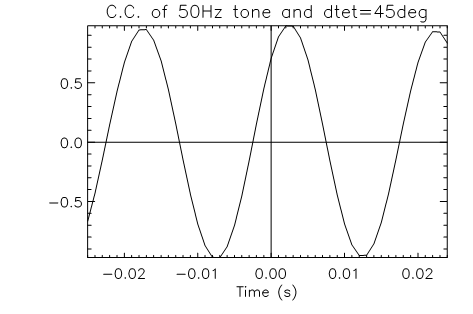
\includegraphics[width=0.9 \columnwidth]{figures/crosscorr.png}
	\end{center}

\end{columns}
\end{frame}

\begin{frame}{Non-Integrated Signal}{$\theta- t$ space visual analysis }
Example
\begin{itemize}
\item Magnetic coils :$ i=1 \ldots 12 $  eq. spaced in poloidal plane
\item $s_i(t) = \cos(\pi f t + m \theta_i) + noise(\mu=0,\sigma=0.2)$
\end{itemize}
\begin{columns}
\column{0.6\textwidth}
	\begin{center}
	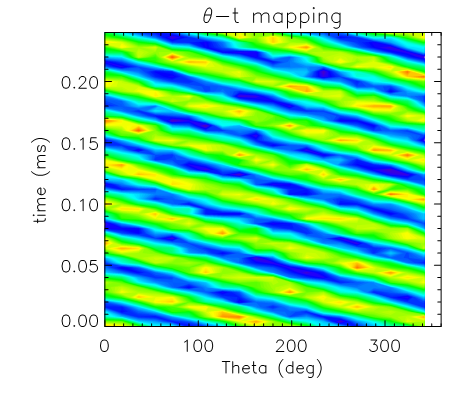
\includegraphics[width=0.8 \columnwidth]{figures/visual-analy.png}
	\end{center}
\column{0.4\textwidth}
\begin{itemize}
\item Wave front propagates clockwise
\item Two periods for fixed t ( m=2)
\item Period $\approx~0.03ms$ $ f~30kHz$
%%(not necessarily the plasma Poloidal rotation frequency…)
\end{itemize}
\end{columns}
\end{frame}

\begin{frame}{Non-Integrated Signal}{MHD Nonrotating Modes }
	\begin{columns}
  	    \column{0.5\textwidth}
		\begin{itemize}
			\item Nonrotating modes are most commonly detected with toroidal arrays of \textbf{ saddle coils}
			\item At low frequencies involved the field perturbation penetrates the vacuum vessel.
		\end{itemize}
	    \column{0.5\textwidth}
		\begin{figure}[ht]
			\begin{center}
				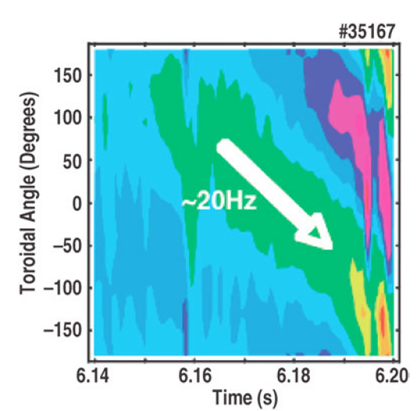
\includegraphics[width=0.6 \columnwidth]{RWM.png}
				\caption{\small  Time evolution of an RWM in JT-60U measured with an array of eight saddle coils.}
			\end{center}
		\end{figure}
 	 \end{columns}
\end{frame}

%Time evolution of an RWM in JT-60U, showing contours of the time derivative of the radial field perturbation measured with a uniformly spaced toroidal array of eight saddle coils
%


%%%%%%%%%%%%%%%%%%%%%%%%%%
\section{Non Inductive Sensors}
\begin{frame}{Non Inductive Sensors}{}
	\begin{columns}
  	    \column{0.45\textwidth}
		\begin{itemize}
			\item Signal has direct Value: $v(t) \propto B(t)$.
			\item Hall Probes are relatively simple and inexpensive. $V_H=\frac{1}{q n} \frac{I_H B}{a}$, \\
			$\frac{1}{q n} $ is \textbf{Hall coefficient}, is a property of each material.
			\item {\color{red} low frequency, low sensivity,  very sensible to radiation!}
		\end{itemize}
	    \column{0.55\textwidth}
			\begin{center}
				\includegraphics[width=0.8 \columnwidth]{Hall.png}

				\includegraphics[width=0.4 \columnwidth]{Hall.jpg}
			\end{center}
 	 \end{columns}
\end{frame}


\begin{frame}{Non Inductive Sensors II}{}
	\begin{columns}
  	    \column{0.4\textwidth}
  	     	\begin{itemize}
			\item Resistive Shunts:
 		     	\begin{itemize}
				\item  Measuring “halo” currents flowing between the plasma and plasma-facing components
			\end{itemize}
			\item Faraday  rotation current  measurements:
		\end{itemize}
	    \column{0.6\textwidth}
			\begin{center}
				\includegraphics[width=0.8 \columnwidth]{Faraday.png}

				{\tiny  Schematic overview of a fiber-optic Faraday rotation measurement device.}
			\end{center}
 	 \end{columns}
\end{frame}

\begin{frame}{Non Inductive Sensors III}{ Faraday effect}
	\begin{center}
		\includegraphics[width=0.8 \columnwidth]{Faraday2.png}
		{\tiny  Scheme of the Faraday effect measurement.}
	\end{center}
\end{frame}

\begin{frame}{Non Inductive Sensors IV}{Fluxgate Magnetometer}
	\begin{columns}
  	    \column{0.5\textwidth} Basic sensor configuration.
		\begin{itemize}
			\item The core is excited by an AC current $I_{exc} $.
			\item  The signal induced in the sense coil $V_{ind}$  at the second harmonic of $I_{exc} $ proportional to the external field $B_{o}$.
		\end{itemize}
  \column{0.5\textwidth}
	\begin{center}
		\includegraphics[width=0.8 \columnwidth]{figures/apprilleflux.png}
%		\includegraphics[width=0.8 \columnwidth]{FluxgateMag.jpg}
		{\tiny  Fluxgate Magnetometer.}
			\includegraphics[width=0.8 \columnwidth]{figures/maghyst.jpg}
	\end{center}
	\end{columns}
\end{frame}

\begin{frame}{Non Inductive Sensors IV}{Fluxgate Magnetometer}
	\begin{columns}
  	    \column{0.5\textwidth}
		\begin{itemize}
			\item Capable of measuring  low frequency DC/ AC fields in the range $10^{-10 }- 10^{-4} T$
			\item  The signal induced in the sense coil $V_{ind}$  at the second harmonic of $I_{exc} $ proportional to the external field $B_{o}$.
			\item Usually double core is adopted
		\end{itemize}
  	     \column{0.5\textwidth}
		\begin{center}
			\includegraphics[width=0.95 \columnwidth]{figures/aprillesignal.png}\\
		{\small Waveform of sensor signal with variable external magnetic (Red curve .}
	\end{center}
	\end{columns}
\end{frame}


 \begin{frame}{Non Inductive Sensors V}{MEMS magnetic field sensors}
	\begin{center}
		\includegraphics[width=0.8 \columnwidth]{mems.pdf}
		{\tiny  MEMS induction based measurement of magnetic fields.}
	\end{center}
\end{frame}

%%%%%%%%%%%%%%%%%%%%%%%%%%
\section{Burning plasma experiments}
\subsection{ITER Burning plasma}

\begin{frame}{Burning plasma experiments}{ITER}
	\begin{columns}
  	    \column{0.6\textwidth}
  		\begin{itemize}
			\item ITER will be the first burning plasma experiment
%		% where all the knowledge on burning plasma diagnostics will converge.
			\item Relative to existing machines (e.g. JET), ITER diagnostic components will be subjected to:
			\begin{itemize}
				\item High $n$ and $\gamma$ fluxes.
				\item $n$ Heating (now essentially zero).
				\item High fluxes of energetic neutral particles.
				\item Long pulse lengths.
			\end{itemize}
		\end{itemize}
%%	High neutron and gamma fluxes (up to x10)
%%Neutron heating (now essentially zero)
%%High fluxes of energetic neutral particles from charge-exchange processes (up to x5)
%%Long pulse lengths (up to x100)
%%High neutron fluence (> x 106)
%		\end{itemize}
  	    \column{0.4\textwidth}
			\begin{center}
				\includegraphics[width=0.8  \columnwidth]{ITER.png}
			\end{center}
 	 \end{columns}
\end{frame}

\subsection{ITER Diagnotics}
\begin{frame}{ITER diagnostics}{Functional requirements}
		Provide accurate measurements of plasma behavior and performance.

  	\begin{itemize}
		\item  3 categories of measurement parameters.
	\end{itemize}
	\begin{tabular}{|c|p{4 cm}|p{4 cm}|}
		\hline
		\textbf {Group}& \textbf {Description} & \textbf {Machine operation? }\\\hline
		1 & Machine protection and Basic machine control & \textit{Advanced} operation unable  without  this\\\hline
		1b & advanced plasma control & Unable  without  \\\hline
		2& Evaluation and physics studies & Able  without  \\\hline
	\end{tabular}
%  		\begin{itemize} %enumerate
%			\item  1 Machine protection and Basic machine control
%	(machine operation unable  without  this group)
%.			\item 1b advanced plasma control
%	(machine \textbf{advanced} operation unable  without  this group)
%			\item 2 2 evaluation and physics studies
%	(machine operation able  without  this group.
%		\end{itemize}
\end{frame}

\begin{frame}{ITER diagnostics}{Magnetic Set}
Total \~ 1700 sensors, 19 types,  $>300\,km$ of cable
	\begin{center}
		\includegraphics[width=0.7 \textheight]{tableIter.png}
	\end{center}
\end{frame}

\begin{frame}{ITER diagnostics}{Poloidal Magnetic Set}
	\begin{center}
		\includegraphics[height=0.8 \textheight]{poloidalIter.png}

	\end{center}
\end{frame}


%%%%%%%%%%%%%%%%%%%%%%%%%%

%\section*{Summary}

%\begin{frame}{Summary}
%
%  % Keep the summary *very short*.
%  \begin{itemize}
%  \item
%    The \alert{first main message} of your talk in one or two lines.
%  \item
%    The \alert{second main message} of your talk in one or two lines.
%  \item
%    Perhaps a \alert{third message}, but not more than that.
%  \end{itemize}
%
%  % The following outlook is optional.
%  \vskip0pt plus.5fill
%  \begin{itemize}
%  \item
%    Outlook
%    \begin{itemize}
%    \item
%      Something you haven't solved.
%    \item
%      Something else you haven't solved.
%    \end{itemize}
%  \end{itemize}
%\end{frame}


%\frame{
%\begin{figure}
%\rule{5cm}{5cm}
%\caption{Test}
%\end{figure}
%}

\begin{frame}{Structure of Magnetosphere}{Earth Fields}
	\begin{center}
		\includegraphics[height=0.85 \textheight]{magsphere.png}
	\end{center}
\end{frame}

\begin{frame}{Magnetosphere}{Plasma Diagnostic}
	\begin{center}
		\includegraphics[height=0.85 \textheight]{aurora1.jpg}
	\end{center}
\end{frame}

% All of the following is optional and typically not needed.
\appendix
\section<presentation>*{\appendixname}
\subsection<presentation>*{Further Reading}

\begin{frame}[allowframebreaks]
  \frametitle<presentation>{Further Reading}

  \begin{thebibliography}{10}

  \beamertemplatebookbibitems
  % Start with overview books.

  \bibitem{Hutchinson 2005}
     I.~ H.~ Hutchinson
    \newblock {\em Principles of Plasma Diagnostics}.
    \newblock Cambridge University Press, 2005.


  \beamertemplatearticlebibitems
  % Followed by interesting articles. Keep the list short.

  \bibitem{E. J. Strait 2008}
    E.~ J.~ Strait et al.
    \newblock  Plasma Diagnostics for Magnetic Fusion Research, ch. 2.
    \newblock {\em Fusion Science and Technology, special Issue} ,Vol. 53, No. 2, February 2008
  \bibitem{Alan Wootton 2008}
    A.~ Wootton
    \newblock  Magnetic Fields and Magnetic Diagnostics for Tokamak Plasmas, 2008,
\href{http://web2.ph.utexas.edu/~iheds/magneticfieldsinatokamak.pdf}{\nolinkurl{web2.ph.utexas.edu/\~iheds/magneticfieldsinatokamak.pdf}}

    %    \newblock {\em Fusion Science and Technology, special Issue} ,Vol. 53, No. 2, February 2008

%  \bibitem{Someone2000}
%    S.~Someone.
%    \newblock On this and that.
%    \newblock {\em Journal of This and That}, 2(1):50--100,
%    2000.
  \end{thebibliography}
\end{frame}

\end{document}
